%%____________________________________________________________________________||
\section{Kinematic distributions for the signal region}
\label{sec:kisigplot}

This appendix shows distributions of events in the signal region in
each \scalht bin in each symmetric and asymmetric \njet bin for each
process as functions of 7 different variables, \ie, \alphat, \mht,
\bdphi, \met, the lead jet $\PT$, the second hardest jet $\PT$, and
\nb.

These distributions are shown in 14 figures from Figs.~\ref{c150107_s150318_f015_alphaT_100}-\ref{c150107_s150318_f015_nbjets_40}. The distributions of each variable
are shown in two figures: one for symmetric \njet bins and the other for
asymmetric \njet bins. Each figure contains 28 panels, each shows the
distribution in the specific \scalht bin and \njet bin for all
processes. These panels are arranged in 4 columns, for 4 different \njet
bins, and 7 rows, for 7 different \scalht bins, and share the axes.
\footnote{This type of data visualisation is called \textit{Trellis
Graphics} (\url{http://ect.bell-labs.com/sl/project/trellis/wwww.html}),
which was originally developed at the Bell Labs in 1990s. Trellis
Graphics is particularly useful for examining multivariate categorical
data \eg to find patters or correlations.}


In these figures, the event selection for the signal region described
in Section \ref{sec:selection} and summarised in tables
\ref{tab:pre-selections}, \ref{tab:alphat-thresholds}, and
\ref{tab:sr-selections} are applied. As described in Section
\ref{sec:preSelection}, the events in the symmetric \njet bins have
the second hardest jet with $\PT$ greater than 100\gev. The events in
the asymmetric \njet bins have the second hardest jet with $\PT$
between 40 and 100\gev.

From these figures, \eg the \nb distributions in Figs.
\ref{c150107_s150318_f015_nbjets_100} and
\ref{c150107_s150318_f015_nbjets_40}, it can be seen that many \scalht
and \njet bins do not contain a multijet event. However, some bins do
contain many multijet events. For example, in Fig.
\ref{c150107_s150318_f015_nbjets_40}, the bin for $350 < \scalht <
400\gev$ and $\njet = 3$ (the panel in the 4th row from the top and
the 2nd column from the left) has many multijet events at $\nb = 0$.
The origin of these multijet events will be clearer in distributions
shown in very fine bins of a histogram. For example, the panel in the
same position in Fig.~\ref{c150107_s150318_f015_biasedDPhi_40} shows
the distribution of the same set of events in very fine bins of
\bdphi. There, all multijet events are in a single bin of \bdphi.
These multijet events correspond to one MC event, weighed by a large
cross section of QCD. In Figures
\ref{c150107_s150318_f015_biasedDPhi_100} and
\ref{c150107_s150318_f015_biasedDPhi_40}, nearly all entries from
multijet events are very tall and contained in isolated bins \bdphi,
which indicates that these multijet events correspond a small number
of MC events.

Event filters and calibrations in the event reconstruction were still
actively developed when MC samples used in this note were generated.
We expect that many of these multijet events still we find in the
signal region will be removed when these filters or calibrations are
well tuned for Run~2 data.

On the other hand, as can be seen in Figure
\ref{c150107_s150318_f015_biasedDPhi_100}, many multijet events reside
in slightly above the cut applied on \bdphi in the highest \scalht and
high \njet bins. If these multijet events persist after the filters and
calibrations are tuned, they can be removed by raising the value of
\bdphi cut.





\begin{figure}[!h]
\centering
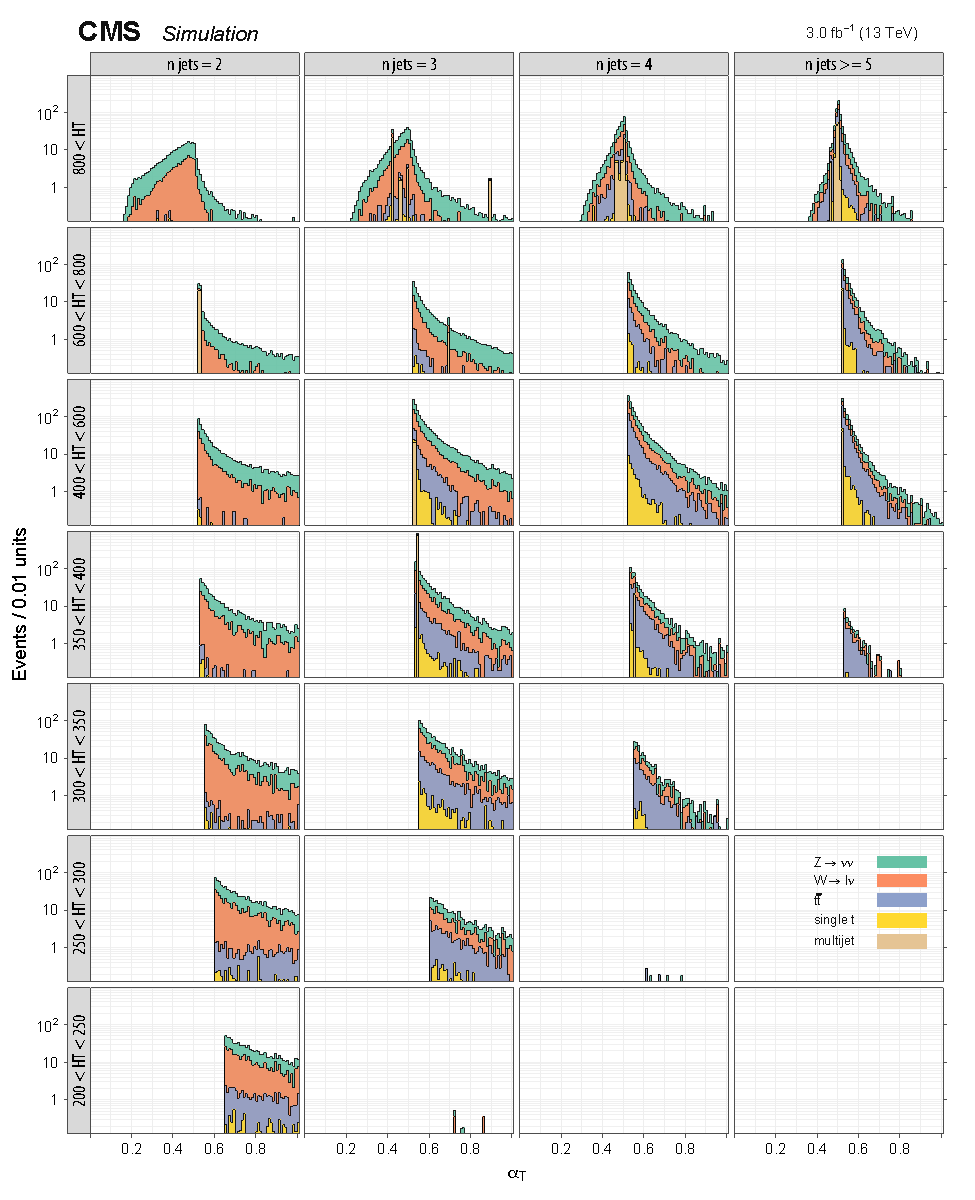
\includegraphics[scale=0.95]{figures/kiplots/c150107_s150318_f015_alphaT_100}
\caption{\textbf{\boldmath The \alphat distributions, symmetric \njet
bins:} The \alphat distributions of the events in the signal region in
each \scalht bin in each symmetric \njet bin for each process. Panels in
different rows show events in different \scalht bins. Panels in
different columns show events in different symmetric \njet bins.
Different processes are shown in different colors (or gray scales).}
\label{c150107_s150318_f015_alphaT_100}
\end{figure}

\begin{figure}[!h]
\centering
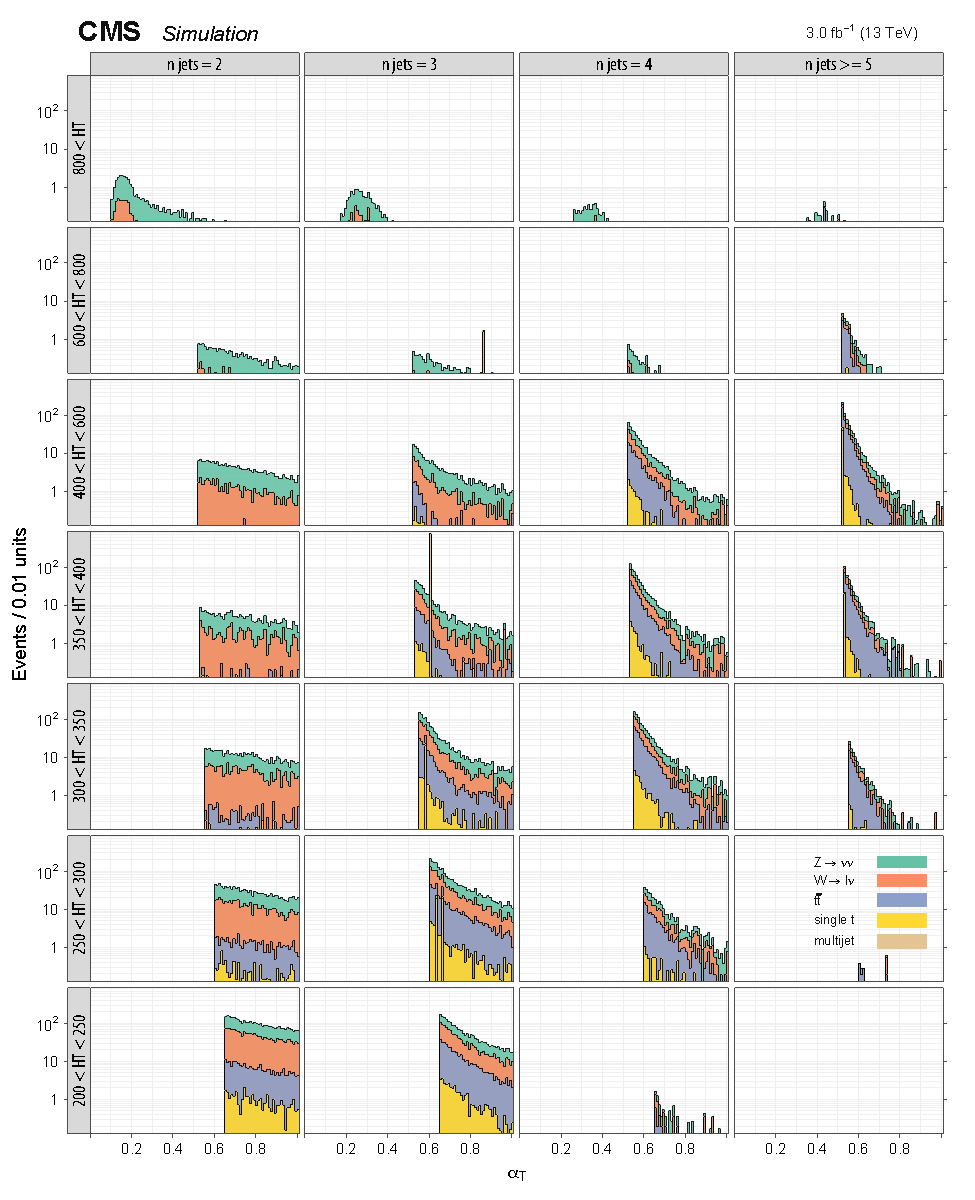
\includegraphics[scale=0.95]{figures/kiplots/c150107_s150318_f015_alphaT_40}
\caption{\textbf{\boldmath The \alphat distributions, asymmetric \njet
bins:} The \alphat distributions of the events in the signal region in
each \scalht bin in each asymmetric \njet bin for each process. Panels
in different rows show events in different \scalht bins. Panels in
different columns show events in different asymmetric \njet bins.
Different processes are shown in different colors (or gray scales).}
\label{c150107_s150318_f015_alphaT_40}
\end{figure}

\begin{figure}[!h]
\centering
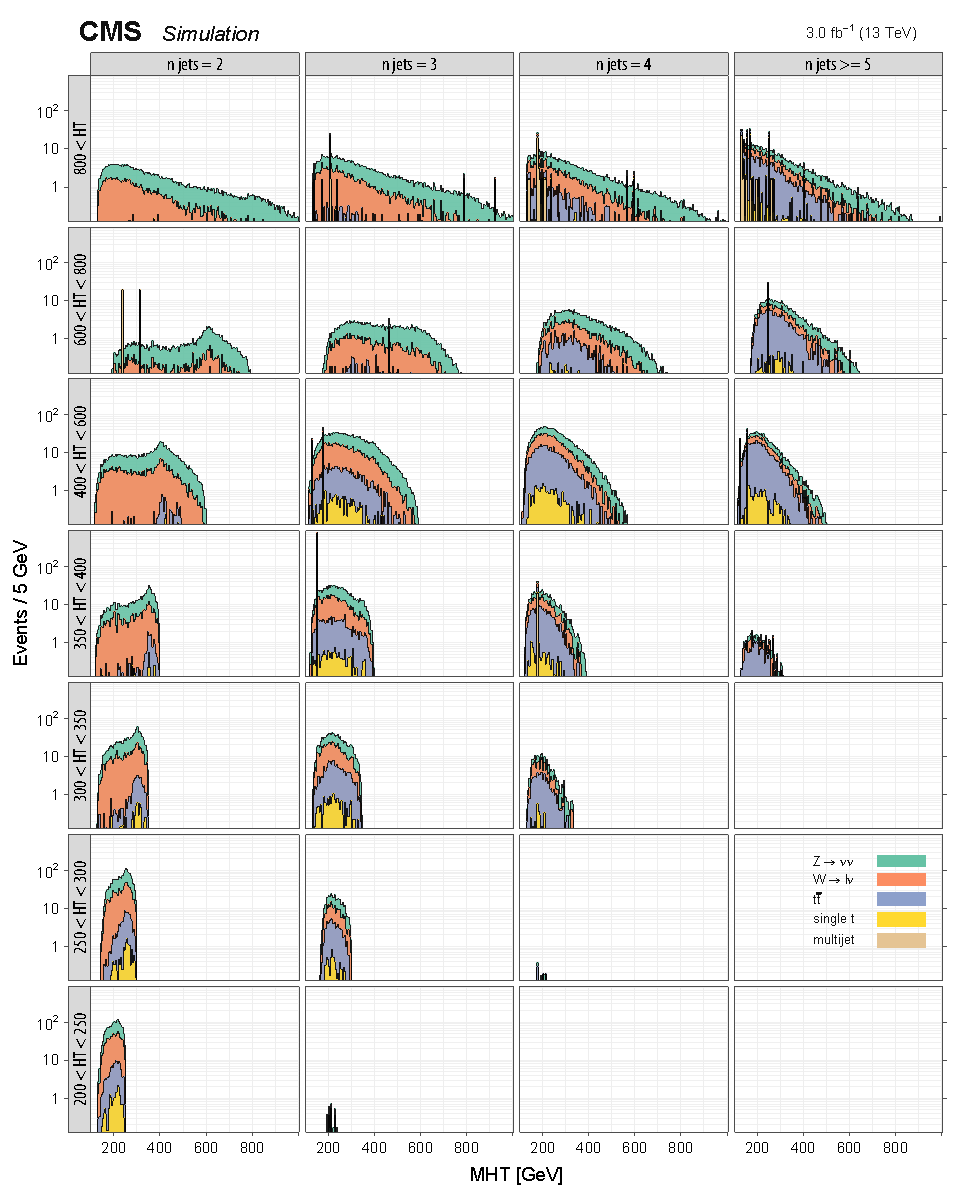
\includegraphics[scale=0.95]{figures/kiplots/c150107_s150318_f015_MHT_100}
\caption{\textbf{\boldmath The \mht distributions, symmetric \njet
bins:} The \mht distributions of the events in the signal region in each
\scalht bin in each symmetric \njet bin for each process. Panels in
different rows show events in different \scalht bins. Panels in
different columns show events in different symmetric \njet bins.
Different processes are shown in different colors (or gray scales).}
\label{c150107_s150318_f015_MHT_100}
\end{figure}

\begin{figure}[!h]
\centering
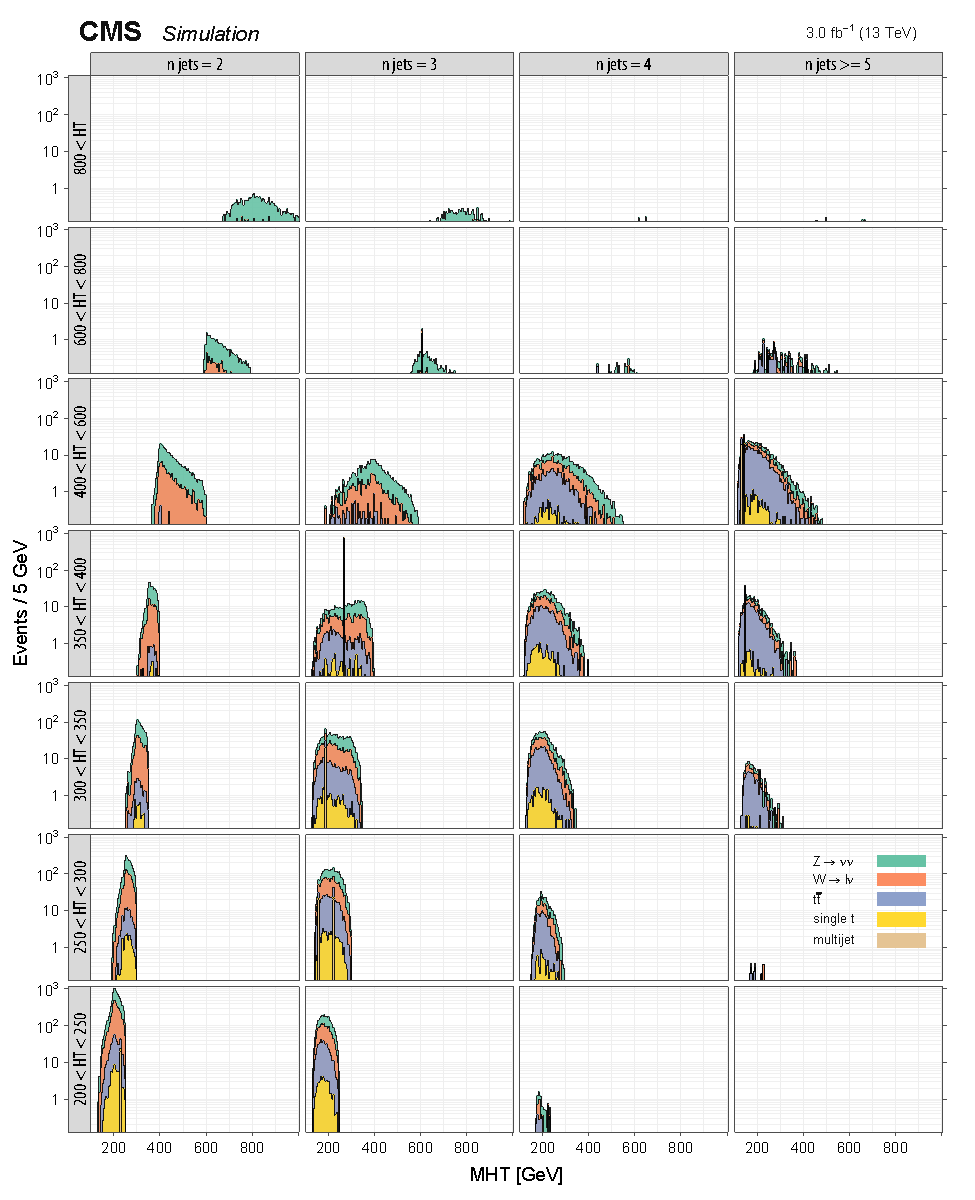
\includegraphics[scale=0.95]{figures/kiplots/c150107_s150318_f015_MHT_40}
\caption{\textbf{\boldmath The \mht distributions, asymmetric \njet
bins:} The \mht distributions of the events in the signal region in each
\scalht bin in each asymmetric \njet bin for each process. Panels in
different rows show events in different \scalht bins. Panels in
different columns show events in different asymmetric \njet bins.
Different processes are shown in different colors (or gray scales).}
\label{c150107_s150318_f015_MHT_40}
\end{figure}

\begin{figure}[!h]
\centering
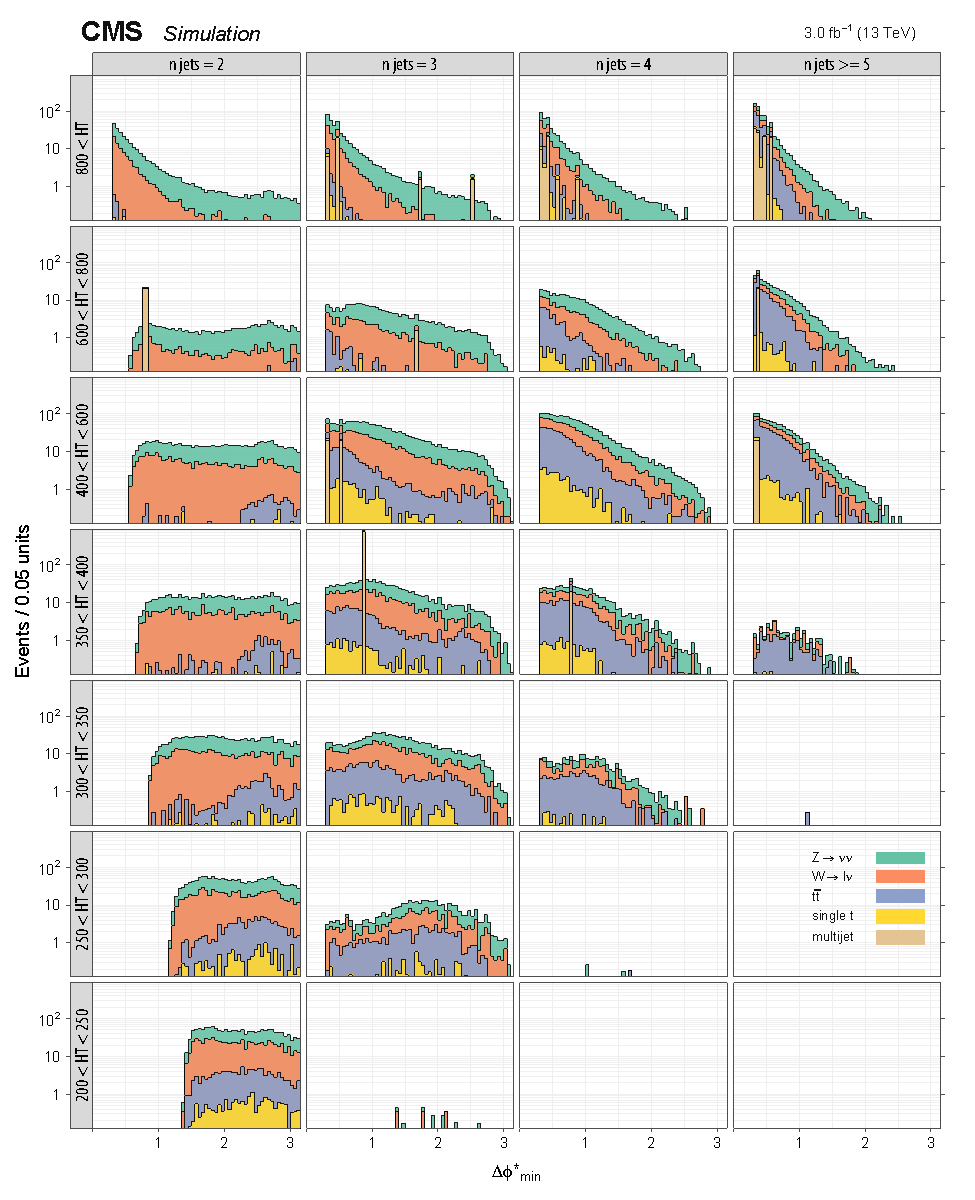
\includegraphics[scale=0.95]{figures/kiplots/c150107_s150318_f015_biasedDPhi_100}
\caption{\textbf{\boldmath The \bdphi distributions, symmetric \njet
bins:} The \bdphi distributions of the events in the signal region in
each \scalht bin in each symmetric \njet bin for each process. Panels in
different rows show events in different \scalht bins. Panels in
different columns show events in different symmetric \njet bins.
Different processes are shown in different colors (or gray scales).}
\label{c150107_s150318_f015_biasedDPhi_100}
\end{figure}

\begin{figure}[!h]
\centering
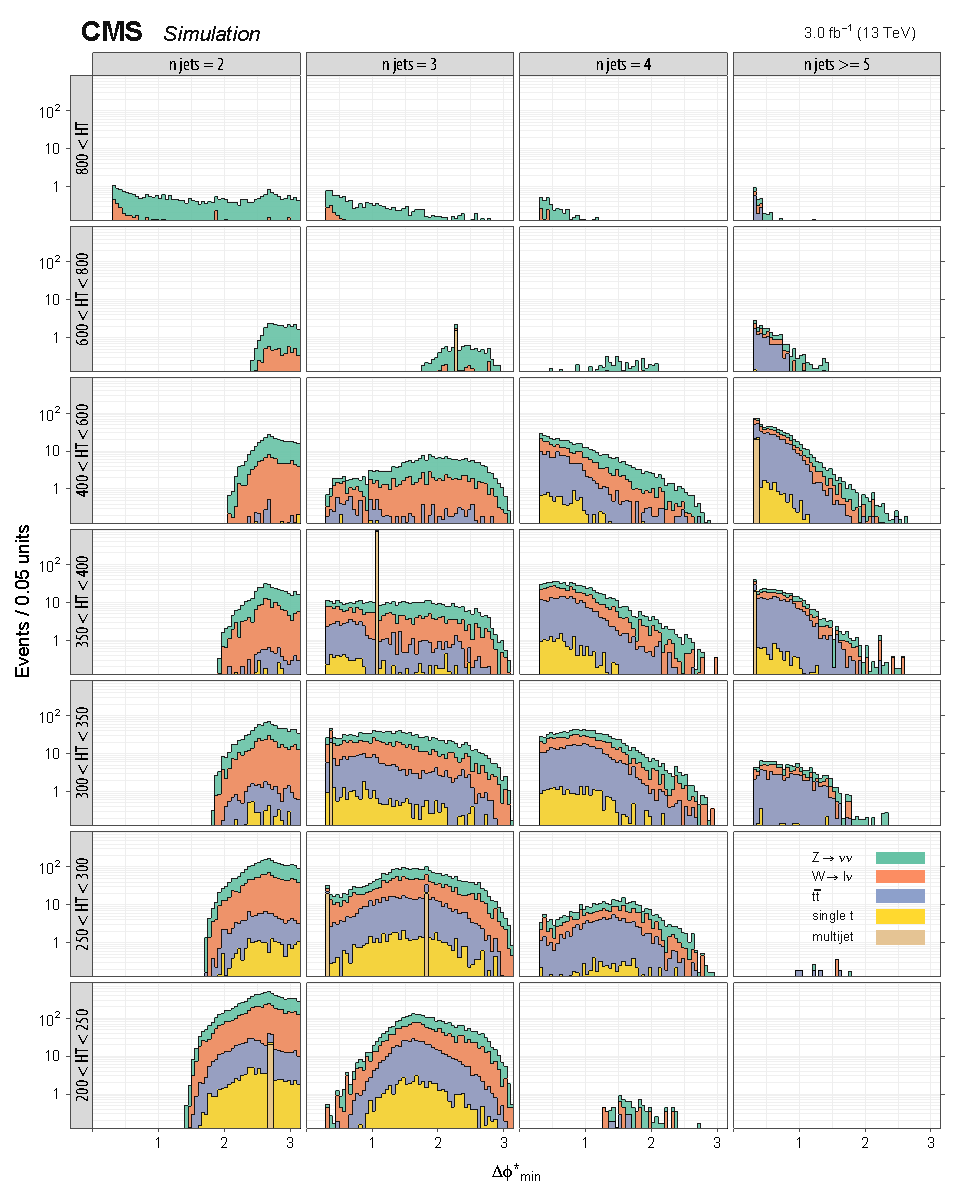
\includegraphics[scale=0.95]{figures/kiplots/c150107_s150318_f015_biasedDPhi_40}
\caption{\textbf{\boldmath The \bdphi distributions, asymmetric \njet
bins:} The \bdphi distributions of the events in the signal region in
each \scalht bin in each asymmetric \njet bin for each process. Panels
in different rows show events in different \scalht bins. Panels in
different columns show events in different asymmetric \njet bins.
Different processes are shown in different colors (or gray scales).}
\label{c150107_s150318_f015_biasedDPhi_40}
\end{figure}

\begin{figure}[!h]
\centering
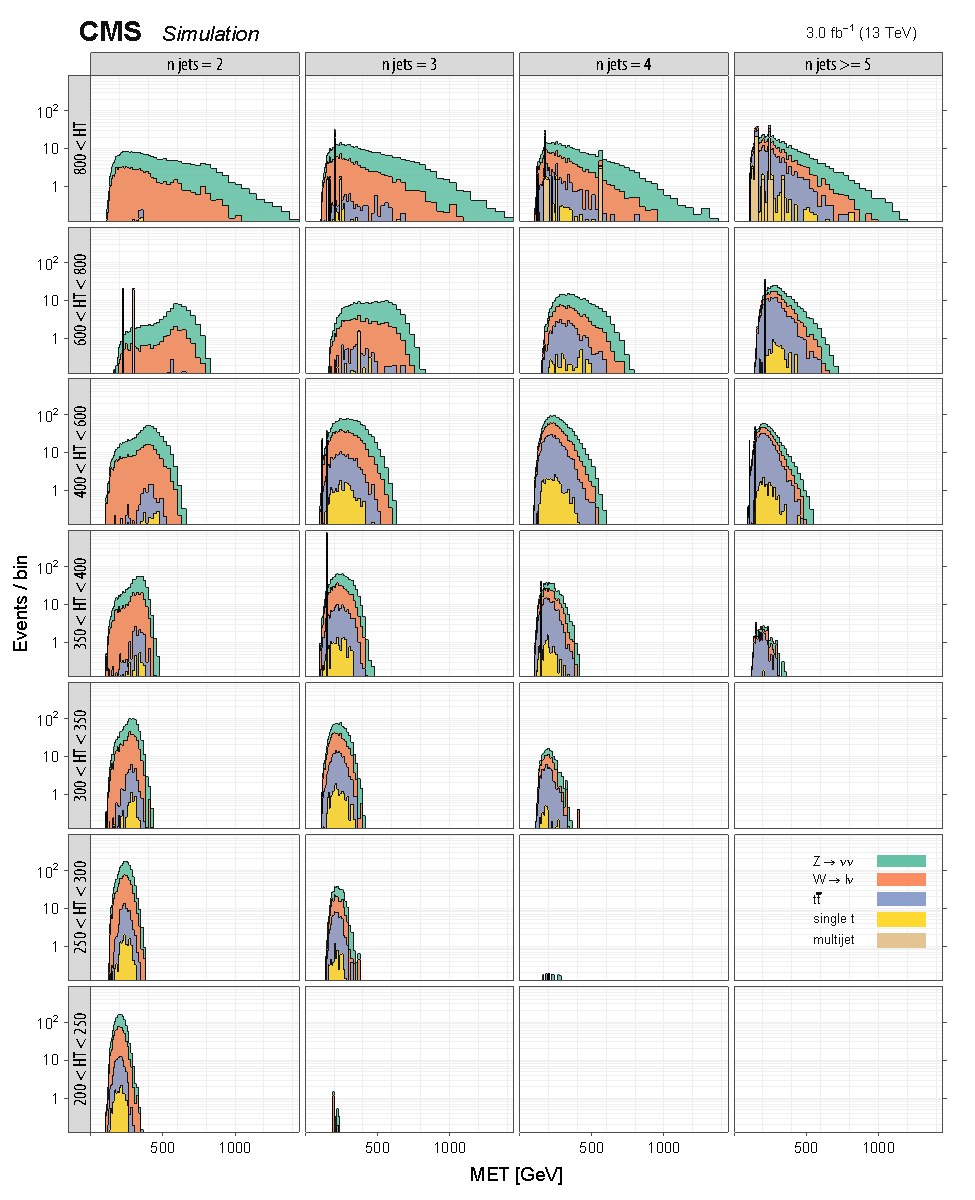
\includegraphics[scale=0.95]{figures/kiplots/c150107_s150318_f015_MET_100}
\caption{\textbf{\boldmath The \met distributions, symmetric \njet
bins:} The \met distributions of the events in the signal region in each
\scalht bin in each symmetric \njet bin for each process. Panels in
different rows show events in different \scalht bins. Panels in
different columns show events in different symmetric \njet bins.
Different processes are shown in different colors (or gray scales).}
\label{c150107_s150318_f015_MET_100}
\end{figure}

\begin{figure}[!h]
\centering
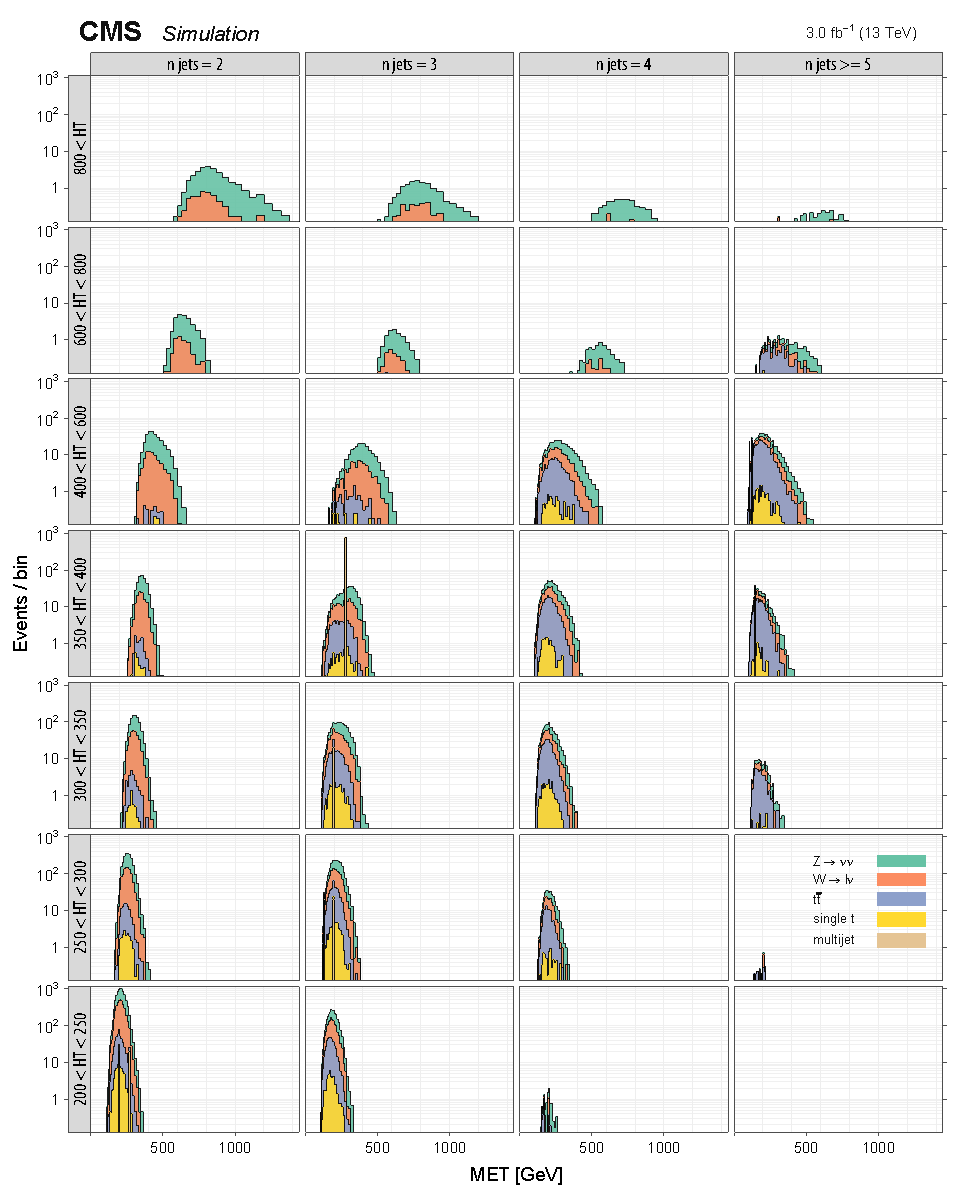
\includegraphics[scale=0.95]{figures/kiplots/c150107_s150318_f015_MET_40}
\caption{\textbf{\boldmath The \met distributions, asymmetric \njet
bins:} The \met distributions of the events in the signal region in each
\scalht bin in each asymmetric \njet bin for each process. Panels in
different rows show events in different \scalht bins. Panels in
different columns show events in different asymmetric \njet bins.
Different processes are shown in different colors (or gray scales).}
\label{c150107_s150318_f015_MET_40}
\end{figure}

\begin{figure}[!h]
\centering
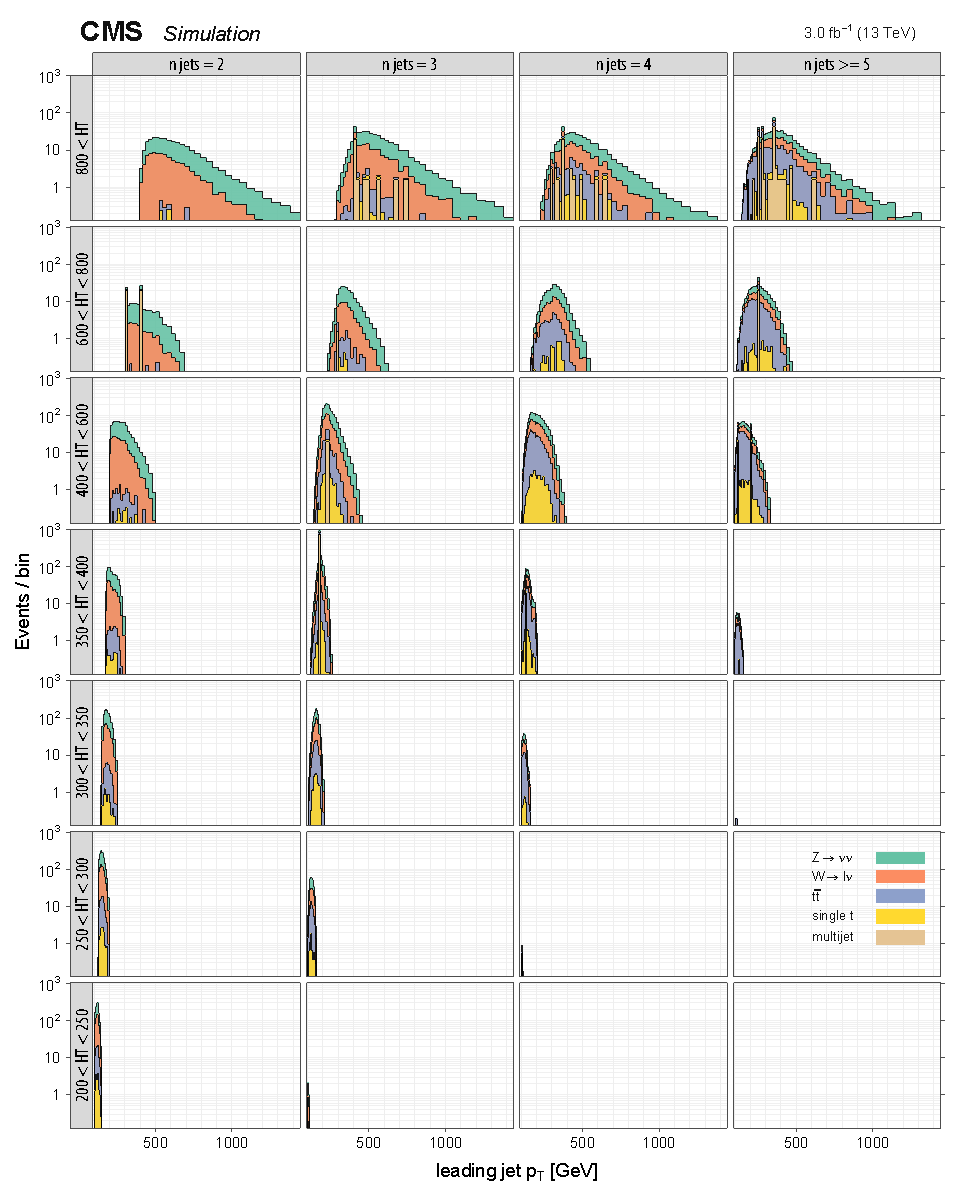
\includegraphics[scale=0.95]{figures/kiplots/c150107_s150318_f015_jet_pt_0_100}
\caption{\textbf{\boldmath The lead jet $\PT$ distributions, symmetric
\njet bins:} The lead jet $\PT$ distributions of the events in the
signal region in each \scalht bin in each symmetric \njet bin for each
process. Panels in different rows show events in different \scalht bins.
Panels in different columns show events in different symmetric \njet
bins. Different processes are shown in different colors (or gray
scales).} \label{c150107_s150318_f015_jet_pt_0_100}
\end{figure}

\begin{figure}[!h]
\centering
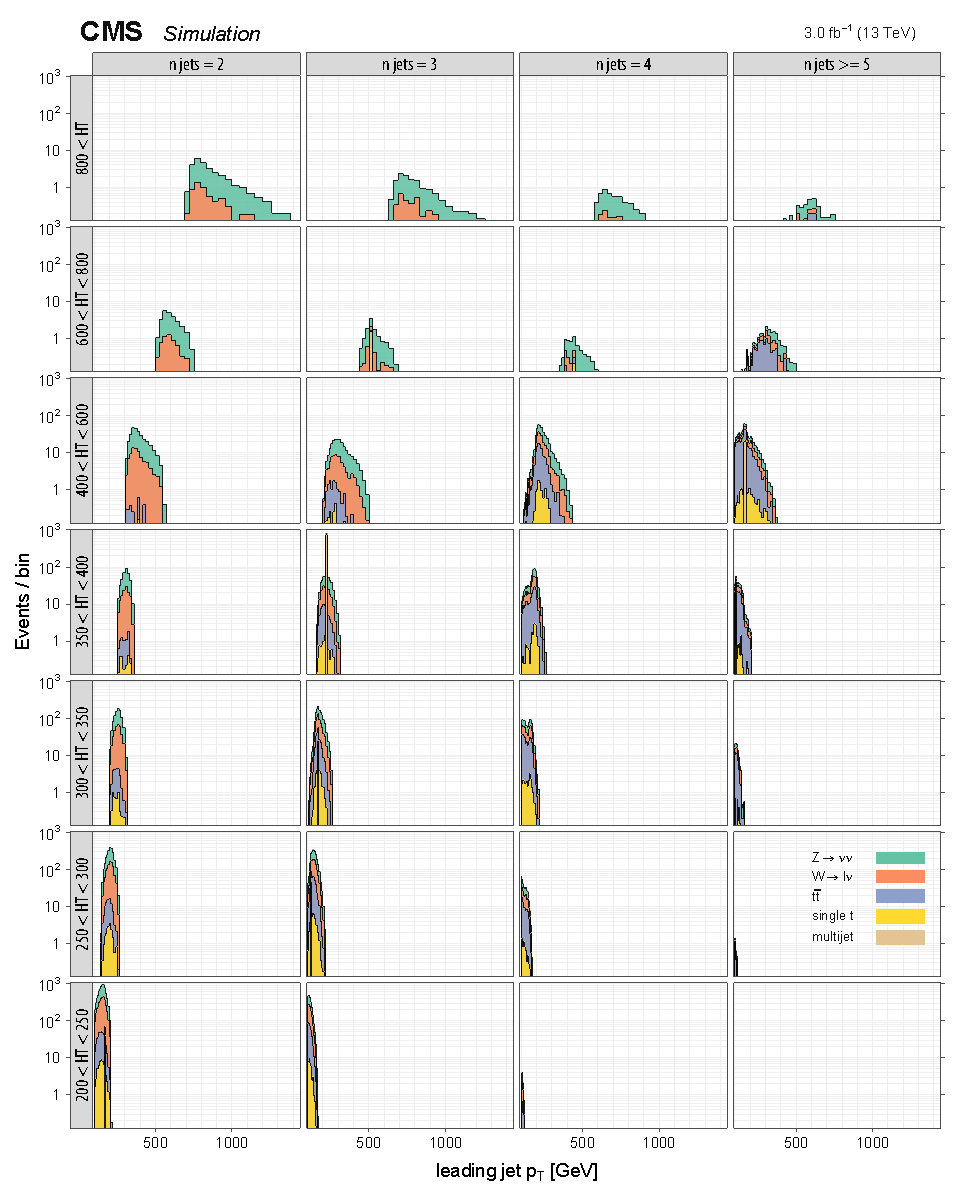
\includegraphics[scale=0.95]{figures/kiplots/c150107_s150318_f015_jet_pt_0_40}
\caption{\textbf{\boldmath The lead jet $\PT$ distributions, symmetric
\njet bins:} The lead jet $\PT$ distributions of the events in the
signal region in each \scalht bin in each asymmetric \njet bin for each
process. Panels in different rows show events in different \scalht bins.
Panels in different columns show events in different asymmetric \njet
bins. Different processes are shown in different colors (or gray
scales).} \label{c150107_s150318_f015_jet_pt_0_40}
\end{figure}

\begin{figure}[!h]
\centering
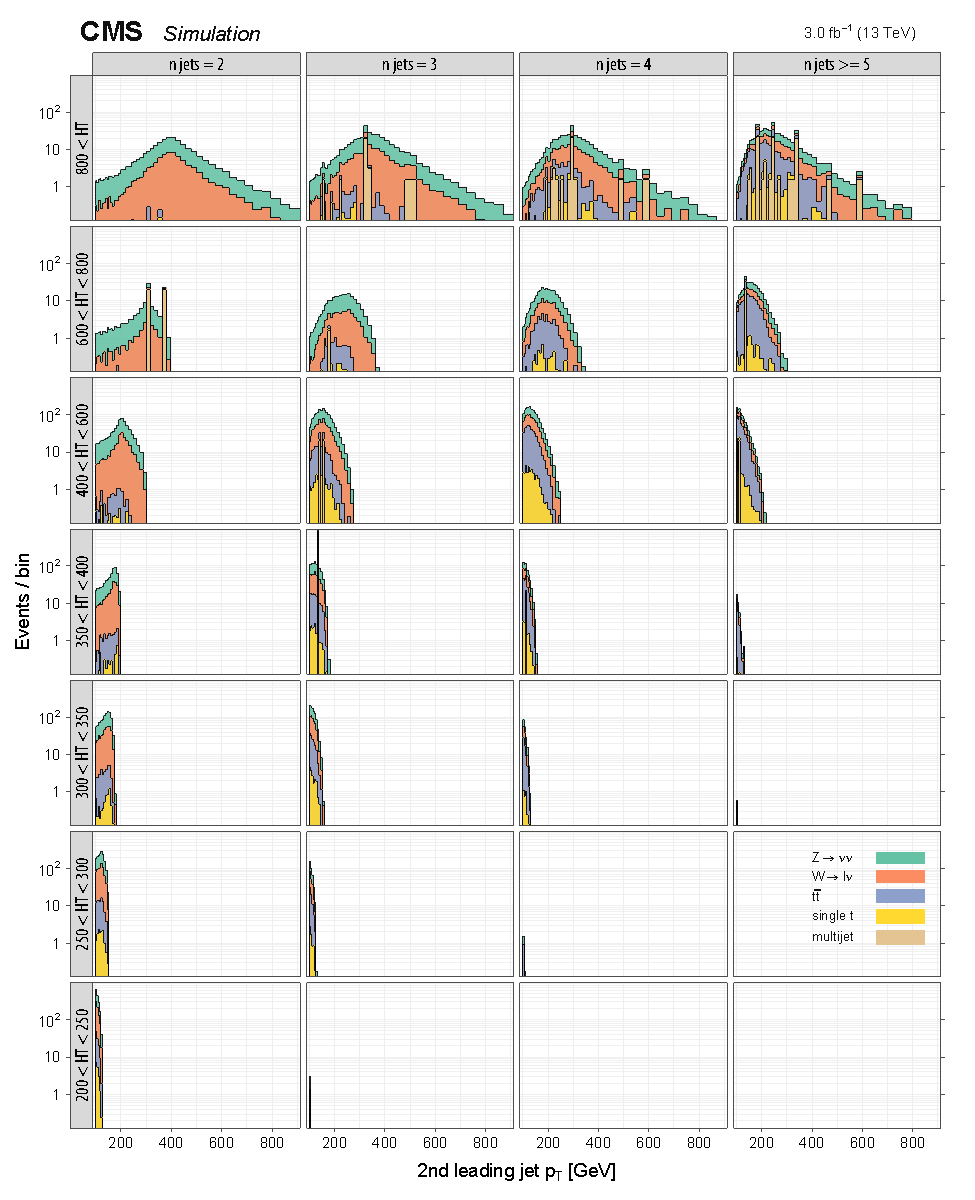
\includegraphics[scale=0.95]{figures/kiplots/c150107_s150318_f015_jet_pt_1_100}
\caption{\textbf{\boldmath The second hardest jet $\PT$ distributions,
symmetric \njet bins:} The second hardest jet $\PT$ distributions of the
events in the signal region in each \scalht bin in each symmetric \njet
bin for each process. Panels in different rows show events in different
\scalht bins. Panels in different columns show events in different
symmetric \njet bins. Different processes are shown in different colors
(or gray scales).} \label{c150107_s150318_f015_jet_pt_1_100}
\end{figure}

\begin{figure}[!h]
\centering
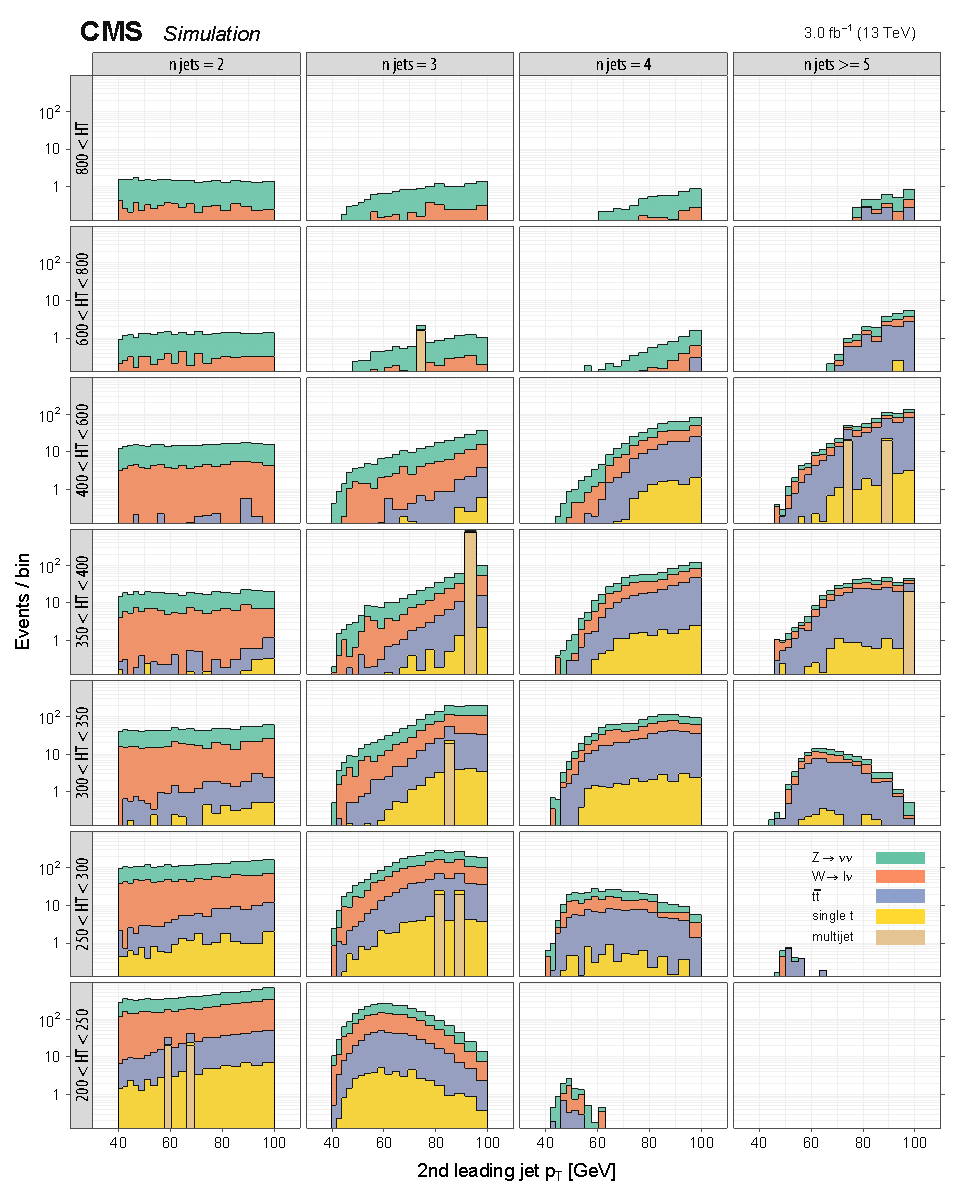
\includegraphics[scale=0.95]{figures/kiplots/c150107_s150318_f015_jet_pt_1_40}
\caption{\textbf{\boldmath The second hardest jet $\PT$ distributions,
asymmetric \njet bins:} The second hardest jet $\PT$ distributions of
the events in the signal region in each \scalht bin in each asymmetric
\njet bin for each process. Panels in different rows show events in
different \scalht bins. Panels in different columns show events in
different asymmetric \njet bins. Different processes are shown in
different colors (or gray scales).}
\label{c150107_s150318_f015_jet_pt_1_40}
\end{figure}

\begin{figure}[!h]
\centering
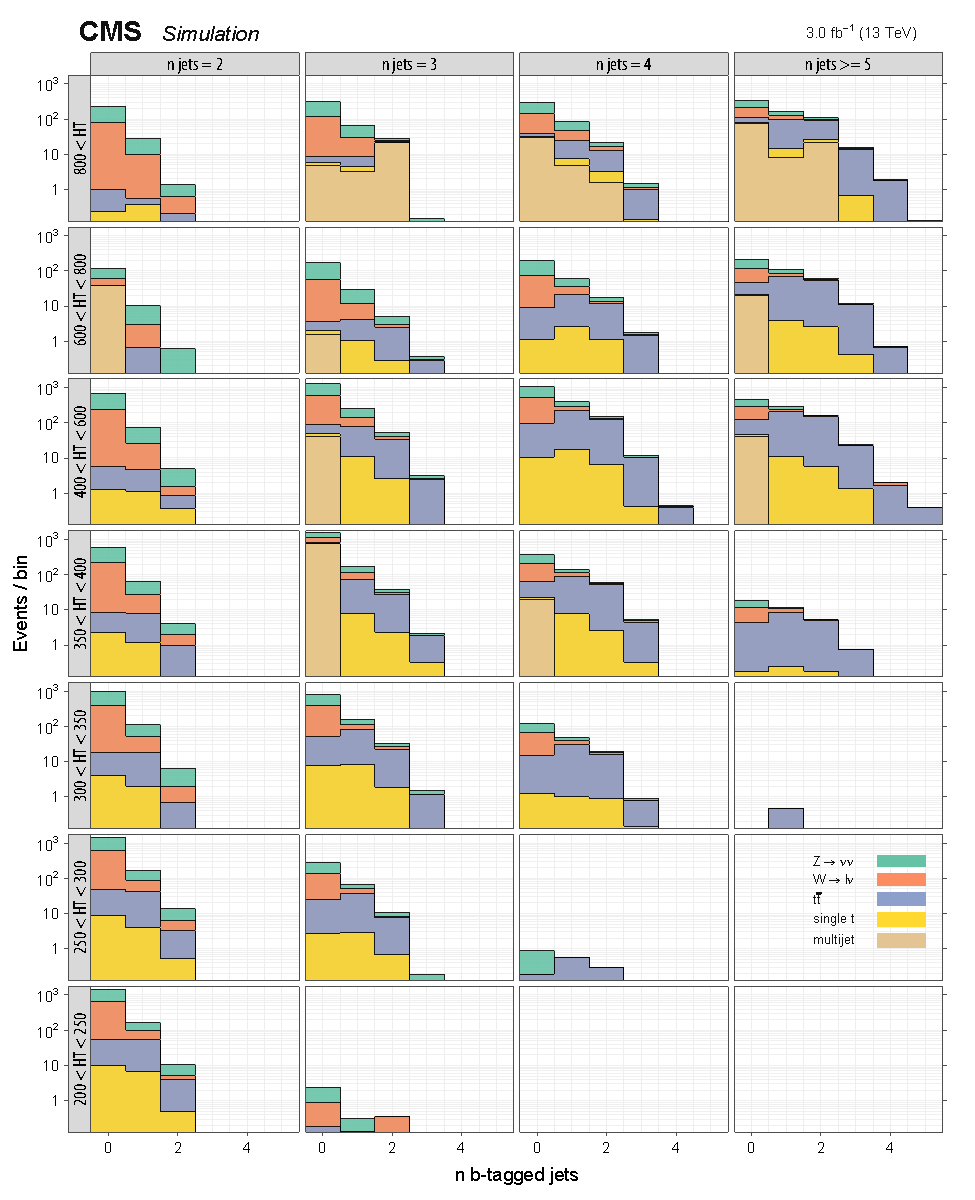
\includegraphics[scale=0.95]{figures/kiplots/c150107_s150318_f015_nbjets_100}
\caption{\textbf{\boldmath The \nb distributions, symmetric \njet bins:}
The $\nb$ distributions of the events in the signal region in each
\scalht bin in each symmetric \njet bin for each process. Panels in
different rows show events in different \scalht bins. Panels in
different columns show events in different symmetric \njet bins.
Different processes are shown in different colors (or gray scales).}
\label{c150107_s150318_f015_nbjets_100}
\end{figure}

\begin{figure}[!h]
\centering
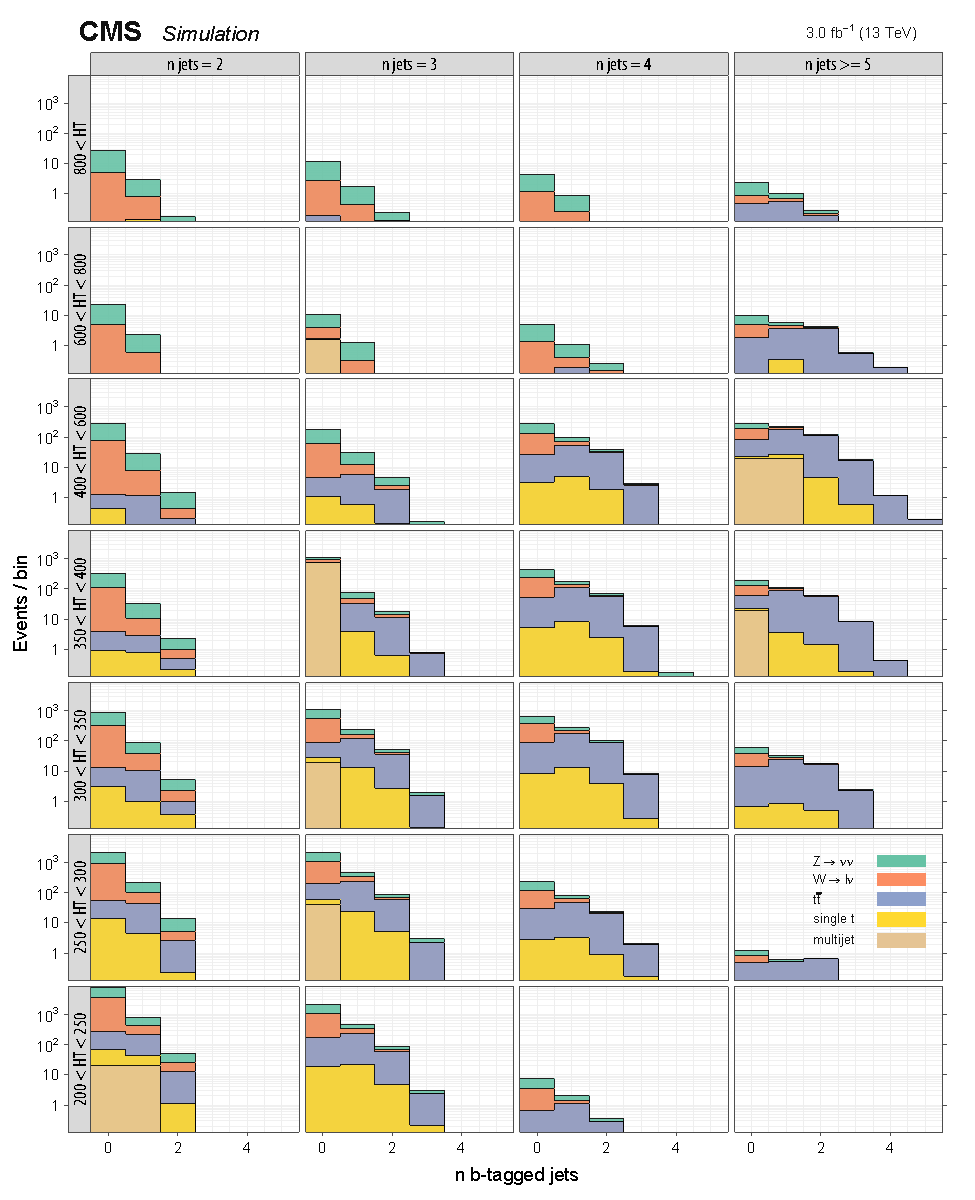
\includegraphics[scale=0.95]{figures/kiplots/c150107_s150318_f015_nbjets_40}
\caption{\textbf{\boldmath The \nb distributions, asymmetric \njet bins:}
The $\nb$ distributions of the events in the signal region in each
\scalht bin in each asymmetric \njet bin for each process. Panels in
different rows show events in different \scalht bins. Panels in
different columns show events in different asymmetric \njet bins.
Different processes are shown in different colors (or gray scales).}
\label{c150107_s150318_f015_nbjets_40}
\end{figure}

%%____________________________________________________________________________||

